\appendix
\etocdepthtag.toc{appendix} % 여기서부터 부록 시작임을 태그 지정
\section*{\Large Appendix}

% \setcounter{figure}{0}
% \setcounter{table}{0}
% \renewcommand{\thefigure}{A.\arabic{figure}}
% \renewcommand{\thetable}{A.\arabic{table}}

%%%%%%%%%%%% TABLE OF CONTENTS %%%%%%%%%%%% 
\makeatletter
\newcommand{\appendix@noopaddcontentsline}[3]{}
\let\appendix@origsection\section
\renewcommand{\section}{\@ifstar\appendix@origsection\appendix@section}
\newcommand{\appendix@section}[1]{%
  \let\appendix@savedaddcontentsline\addcontentsline
  \let\addcontentsline\appendix@noopaddcontentsline
  \appendix@origsection{#1}%
  \let\addcontentsline\appendix@savedaddcontentsline
  \phantomsection
  \addcontentsline{toc}{section}{\protect\numberline{\thesection}#1}%
}
\let\appendix@origsubsection\subsection
\renewcommand{\subsection}{\@ifstar\appendix@origsubsection\appendix@subsection}
\newcommand{\appendix@subsection}[1]{%
  \let\appendix@savedaddcontentsline\addcontentsline
  \let\addcontentsline\appendix@noopaddcontentsline
  \appendix@origsubsection{#1}%
  \let\addcontentsline\appendix@savedaddcontentsline
  \phantomsection
  \addcontentsline{toc}{subsection}{\protect\numberline{\thesubsection}#1}%
}
\makeatother

\etocsetlevel{author}{6}
\etocsetlevel{title}{6}
\etocsettagdepth{main}{none}
\etocsettagdepth{appendix}{subsection}
\makeatletter
{%
\let\section\appendix@origsection
\let\subsection\appendix@origsubsection
\tableofcontents
}
\makeatother

\etocdepthtag.toc{appendix} % 여기서부터 부록 시작임을 태그 지정
%%%%%%%%%%%% TABLE OF CONTENTS %%%%%%%%%%%% 



\clearpage
\section{Training Details}
\label{sec:appendix_experimental_details}
Our primary interest is in transferability, \textit{i.e.}, whether learning a task in one modality improves performance on the corresponding task in the other modality. Thus, for the transferability experiments, our default strategy is to apply LoRA to the Query, Key, Value projection and MLP layers of the transformer blocks, which is  shared across modalities. All other major components, including the image encoder, projector/aligner, language modeling head, and diffusion head, are kept frozen. Across all runs, we use LoRA rank 128, 8-bit AdamW, a global batch size of 128, and bfloat16 training. To enable a fair comparison across architectures, we select models in the 7B--8B parameter range. For quantitative results, we report the best checkpoint from each training run.
For BAGEL~\cite{deng2025bagel}, we use a learning rate of $1\times10^{-4}$ and retain the original dynamic image resizing strategy of the model. For Janus-Pro~\cite{chen2025januspro}, we use the Janus-Pro-7B checkpoint with a learning rate of $4\times10^{-5}$; for both understanding and generation, we preserve the original aspect ratio, resize the longer side to 384 pixels, and pad the shorter side to obtain a $384 \times 384$ input. For Lumina-DiMOO, we use a learning rate of $3\times10^{-6}$; for both understanding and generation, we preserve the original aspect ratio, resize the longer side to 512 pixels, and pad the shorter side to obtain a $512 \times 512$ input. For BLIP3-o~\cite{chen2505blip3}, we use the BLIP3o-8B checkpoint. Since BLIP3-o employs separate transformers for understanding and generation, we fine-tune the corresponding branch for each task. We retain the original image processing strategy of Qwen2.5-VL-7B-Instruct~\cite{bai2025qwen2}, which is used as LLM backbone of BLIP3-o.

\clearpage
\section{Task Details}
\label{sec:appendix_dataset_construction}
\subsection{Counting}
\subsubsection{Dataset detail.} Our \textit{visual instruction tuning dataset} for counting consists of 65.6K images and approximately 200K question-answer pairs. We derive the VQA pairs from the training sets of PixMo-Count~\cite{deitke2025molmo} and PixMo-Points~\cite{deitke2025molmo}.
For counting understanding, we directly adopt the original question-answer pairs from PixMo-Count, as it is originally designed for counting tasks. To scale up the training data, we additionally incorporate samples from PixMo-Points. Since PixMo-Points is a point prediction dataset rather than a counting dataset, we reformulate it for counting by treating the number of points to be predicted as the object count. Note that PixMo-Points originally contains annotations more thank 1K points per image. We find that such extreme cases introduce excessive difficulty during training. To maintain a reasonable difficulty level, we filter out samples whose object count exceeds 20. For \textit{counting-aware generation dataset}, we construct the training set from the same 65.6K images used in the understanding split to ensure a controlled experimental setting. Specifically, we leverage the object count annotations from the understanding training set and use Qwen3-VL~\cite{bai2025qwen3} to generate count-aware generation prompts conditioned on these annotations.
Table~\ref{} presents representative samples from both the counting understanding and generation training sets.


\subsubsection{Understanding evaluation.}
We evaluate counting understanding using 540 QA pairs constructed from the test split of PixMo-Count. Each QA pair explicitly includes both the question and a response template. In particular, the prompt contains a \texttt{Response Example} field that asks the model to place the predicted count inside the markdown markers \texttt{** **}. During evaluation, we first parse the substring enclosed by these markers and compare it with the ground-truth count. If such parsing fails, we fall back to checking whether the ground-truth count appears anywhere in the model output, either as an Arabic numeral or as an English number word. This heuristic allows us to robustly score free-form responses while preserving the intended answer format. An example QA pair is shown below.

\begin{quote}
\textbf{Question:} How many people are there in the image? Response Example: There are \texttt{**<number>**} of people in the image. \\
\textbf{Answer:} There are \texttt{**5**} of people in the image.
\end{quote}


\subsubsection{Generation evaluation.} 
Following the prompt generation protocol of GenEval~\cite{ghosh2023geneval}, 
we construct a total of 90 prompts by combining 10 object classes 
and 9 count words, yielding 90 prompts in total. 
Each prompt follows the template:

\begin{quote}
\texttt{"a photo of \{COUNT\} \{OBJECT\}s"}
\end{quote}

\noindent where \texttt{OBJECT} $\in$ \{\texttt{person, dog, cat, car, 
cup, chair, book, bottle, apple, tie}\} and \texttt{COUNT} $\in$ 
\{\texttt{two, three, four, five, six, seven, eight, nine, ten}\}.

For each prompt, we generate four images with different random seeds 
and report the average accuracy across all generated samples.
To obtain object counts from generated images, we follow same detection-based approach as GenEval~\cite{ghosh2023geneval}.
\begin{table*}[t]
\centering
\label{tab:dataset_examples}
\setlength{\tabcolsep}{6pt}
\resizebox{\textwidth}{!}{%
\begin{tabular}{cccc}
\toprule
{\textbf{Image}} & {\textbf{PixMo QA}} & \textbf{Understanding QA} &{\textbf{Generation Prompt}} \\
\midrule
\addlinespace[4pt]
\raisebox{-0.5\height}{\includegraphics[width=5cm]{example-image-a}} &
\parbox[c]{4cm}{\raggedright\small A blue-toned photograph of a coastal scene with waves.} &
\parbox[c]{4cm}{\raggedright\small Describe the scene.} &
\parbox[c]{6cm}{\raggedright\scriptsize You are given a photograph of a coastal landscape. Please provide a comprehensive description of all visible elements including the water conditions, rock formations, sky color, and any atmospheric effects.} \\
\addlinespace[10pt]
\raisebox{-0.5\height}{\includegraphics[width=5cm]{example-image-a}} &
\parbox[c]{4cm}{\raggedright\small A warm sunset over a desert canyon with sandstone.} &
\parbox[c]{4cm}{\raggedright\small What colors are present?} &
\parbox[c]{6cm}{\raggedright\scriptsize Analyze the following desert landscape image. Identify all color gradients, geological textures, and lighting conditions visible in the scene.} \\
\addlinespace[10pt]
\raisebox{-0.5\height}{\includegraphics[width=5cm]{example-image-a}} &
\parbox[c]{4cm }{\raggedright\small A lush green forest with sunlight filtering through.} &
\parbox[c]{4cm }{\raggedright\small Identify vegetation types.} &
\parbox[c]{6cm}{\raggedright\scriptsize Examine the provided forest photograph and enumerate all distinguishable plant species or vegetation categories. Note the distribution of light and shadow.} \\
\addlinespace[10pt]
\raisebox{-0.5\height}{\includegraphics[width=5cm]{example-image-a}} &
\parbox[c]{4cm }{\raggedright\small A purple-tinted cityscape at twilight with neon.} &
\parbox[c]{4cm }{\raggedright\small Describe the environment.} &
\parbox[c]{6cm}{\raggedright\scriptsize You are presented with a nighttime urban scene. Provide a thorough description covering all visible architectural elements, signage, lighting sources, and human activity.} \\
\addlinespace[4pt]
\bottomrule
\end{tabular}
}% end resizebox
\caption{Examples of counting dataset.}
\end{table*}
\subsection{Spatial Relation}
\subsubsection{Dataset detail.}
This place is for jaewoo!
\begin{table*}[t]
\centering
\label{tab:spatial_example}
\setlength{\tabcolsep}{6pt}
\resizebox{\textwidth}{!}{%
\begin{tabular}{cccc}
\toprule
{\textbf{Image}} & {\textbf{Prompt}} & {\textbf{Image}} & {\textbf{Prompt}} \\
\midrule

\addlinespace[4pt]

\raisebox{-0.5\height}{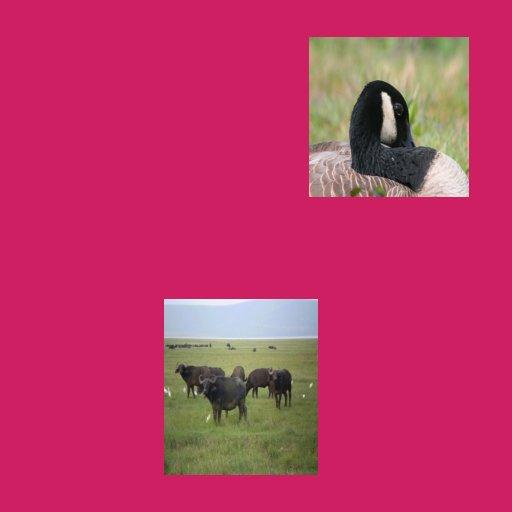
\includegraphics[width=5cm]{x_supple/files/topright1.jpg}} &
\parbox[c]{6cm}{\raggedright\normalsize A blue-toned photograph of a coastal scene with waves. Describe the scene.} &
\raisebox{-0.5\height}{\includegraphics[width=5cm]{example-image-a}} &
\parbox[c]{6cm}{\raggedright\normalsize A warm sunset over a desert canyon with sandstone. What colors are present?} \\

\addlinespace[10pt]

\raisebox{-0.5\height}{\includegraphics[width=5cm]{example-image-a}} &
\parbox[c]{6cm}{\raggedright\normalsize A lush green forest with sunlight filtering through. Identify vegetation types.} &
\raisebox{-0.5\height}{\includegraphics[width=5cm]{example-image-a}} &
\parbox[c]{6cm}{\raggedright\normalsize A purple-tinted cityscape at twilight with neon. Describe the environment.} \\

\addlinespace[10pt]

\raisebox{-0.5\height}{\includegraphics[width=5cm]{example-image-a}} &
\parbox[c]{6cm}{\raggedright\normalsize A lush green forest with sunlight filtering through. Identify vegetation types.} &
\raisebox{-0.5\height}{\includegraphics[width=5cm]{example-image-a}} &
\parbox[c]{6cm}{\raggedright\normalsize A purple-tinted cityscape at twilight with neon. Describe the environment.} \\

\addlinespace[10pt]

\raisebox{-0.5\height}{\includegraphics[width=5cm]{example-image-a}} &
\parbox[c]{6cm}{\raggedright\normalsize A lush green forest with sunlight filtering through. Identify vegetation types.} &
\raisebox{-0.5\height}{\includegraphics[width=5cm]{example-image-a}} &
\parbox[c]{6cm}{\raggedright\normalsize A purple-tinted cityscape at twilight with neon. Describe the environment.} \\
\addlinespace[4pt]

\bottomrule
\end{tabular}
}% end resizebox
\caption{Examples of spatial relation dataset.}
\end{table*}
\subsubsection{Generation evaluation.} 
\begin{figure*}[t]
\centering
\fbox{%
\begin{minipage}{0.96\textwidth}
\vspace{6pt}
\tiny
\setlength{\fboxsep}{2pt}
\renewcommand{\baselinestretch}{0.9}
\noindent
\begin{minipage}[t]{0.48\textwidth}
\ttfamily
1. The dog located in the top-left of a teddy bear.\\
2. The wine glass located in the bottom-right of a kite.\\
3. The couch is located in bottom-left of a cup.\\
4. The laptop can be found to the top-right of a cow.\\
5. The fork is located in top-right of a hair drier.\\
6. The tie can be found to the bottom-left of a baseball bat.\\
7. The stop sign is located in top-right of a fork.\\
8. The bird is located in bottom-left of a skateboard.\\
9. The an apple located in the bottom-right of a tv.\\
10. The train located in the bottom-right of a potted plant.\\
11. The truck can be found to the top-right of a refrigerator.\\
12. The tv remote is located in bottom-right of a cow.\\
13. The bottle can be found to the bottom-left of a train.\\
14. The dog is located in top-right of a cow.\\
15. The skateboard located in the bottom-left of a person.\\
16. The baseball glove is located in bottom-left of an umbrella.\\
17. The dining table located in the top-right of an oven.\\
18. The hot dog can be found to the top-left of a suitcase.\\
19. The bus is located in top-left of a toothbrush.\\
20. The backpack located in the top-right of a sandwich.\\
21. The cake is located in bottom-right of a baseball bat.\\
22. The dog located in the top-left of a tie.\\
23. The suitcase can be found to the bottom-left of a boat.\\
24. The bear located in the bottom-right of a clock.\\
25. The tv remote can be found to the top-right of an umbrella.\\
26. The sports ball can be found to the top-left of an umbrella.\\
27. The train located in the top-right of a dining table.\\
28. The hair drier is located in bottom-right of an elephant.\\
29. The tennis racket can be found to the bottom-left of a spoon.\\
30. The wine glass can be found to the bottom-left of a hot dog.\\
31. The computer mouse can be found to the top-right of a bench.\\
32. The carrot can be found to the top-right of an orange.\\
33. The kite located in the bottom-right of a toothbrush.\\
34. The toaster is located in top-left of a traffic light.\\
35. The cat is located in top-left of a baseball glove.\\
36. The skis located in the top-left of a zebra.\\
37. The stop sign located in the bottom-left of a chair.\\
38. The stop sign located in the bottom-right of a parking meter.\\
39. The hot dog located in the top-left of a skateboard.\\
40. The pizza is located in bottom-left of a computer keyboard.\\
41. The hair drier can be found to the top-left of a toilet.\\
42. The cow can be found to the bottom-right of a stop sign.\\
43. The suitcase is located in top-right of a skis.\\
44. The book located in the bottom-left of a laptop.\\
45. The toothbrush is located in top-left of a pizza.\\
46. The toilet can be found to the top-right of a kite.\\
47. The tie is located in top-right of a sink.\\
48. The bird can be found to the bottom-right of a couch.\\
49. The bed can be found to the bottom-left of a sports ball.\\
50. The an elephant is located in top-left of a surfboard.\\
\end{minipage}
\hfill
\begin{minipage}[t]{0.48\textwidth}
\ttfamily
51. The frisbee can be found to the bottom-left of a motorcycle.\\
52. The vase located in the bottom-right of a fire hydrant.\\
53. The zebra can be found to the top-left of an elephant.\\
54. The bench can be found to the bottom-right of a bear.\\
55. The donut located in the top-left of a bench.\\
56. The frisbee is located in bottom-left of a horse.\\
57. The computer keyboard located in the bottom-right of a snowboard.\\
58. The tv is located in bottom-right of a cow.\\
59. The an elephant is located in top-left of a horse.\\
60. The suitcase can be found to the top-right of a banana.\\
61. The train is located in top-left of an airplane.\\
62. The cat is located in bottom-right of a backpack.\\
63. The backpack is located in bottom-left of a cake.\\
64. The sandwich is located in bottom-left of a knife.\\
65. The bicycle is located in top-right of a parking meter.\\
66. The knife located in the top-left of a suitcase.\\
67. The hot dog located in the bottom-left of a knife.\\
68. The zebra located in the top-left of a parking meter.\\
69. The chair can be found to the bottom-right of a zebra.\\
70. The cow is located in top-left of an airplane.\\
71. The cup can be found to the bottom-right of an umbrella.\\
72. The zebra is located in bottom-left of a computer keyboard.\\
73. The zebra is located in bottom-left of a broccoli.\\
74. The laptop is located in bottom-right of a sports ball.\\
75. The truck can be found to the top-left of a baseball bat.\\
76. The refrigerator is located in top-right of a baseball bat.\\
77. The tv located in the bottom-right of a baseball bat.\\
78. The baseball glove located in the top-left of a bear.\\
79. The refrigerator is located in bottom-right of a scissors.\\
80. The dining table located in the bottom-right of a suitcase.\\
81. The parking meter located in the bottom-right of a broccoli.\\
82. The frisbee located in the bottom-right of a truck.\\
83. The pizza located in the top-left of a banana.\\
84. The bus located in the bottom-left of a boat.\\
85. The cell phone can be found to the bottom-right of a tennis racket.\\
86. The horse located in the top-right of a broccoli.\\
87. The broccoli located in the bottom-left of a bottle.\\
88. The vase can be found to the bottom-left of a horse.\\
89. The bear is located in top-right of a spoon.\\
90. The zebra located in the top-left of a bed.\\
91. The cow can be found to the bottom-left of a laptop.\\
92. The bed located in the top-left of a frisbee.\\
93. The tie located in the top-right of a motorcycle.\\
94. The laptop can be found to the bottom-left of a tv.\\
95. The cell phone can be found to the bottom-left of a chair.\\
96. The couch is located in top-left of a potted plant.\\
97. The clock is located in bottom-left of a tv.\\
98. The couch is located in bottom-right of a vase.\\
99. The donut is located in bottom-left of a cat.\\
100. The couch can be found to the top-left of a toaster.\\
\end{minipage}
\vspace{6pt}
\end{minipage}%
}
\caption{\textbf{Full list of spatial relation evaluation prompts.}
All 100 prompts used for spatial relation evaluation.
Each prompt describes the relative position of two COCO objects using one of the predefined position templates.}
\label{fig:spatial_prompts}
\end{figure*}
We generate 100 prompts describing spatial relationships between two 
objects, following the same prompt format used during training. 
The full list of evaluation prompts is provided in Fig.~\ref{fig:spatial_prompts}.
For each prompt, we generate four images with different random seeds 
and report the average accuracy across all generated samples.

For evaluation, we follow the same detection-based approach as GenEval~\cite{ghosh2023geneval}, obtaining bounding boxes for both objects. 
The relative position between objects is determined by the difference 
between bounding box centroids: if object $A$ is centered at $(x_A, y_A)$ 
and object $B$ is centered at $(x_B, y_B)$, following standard image 
coordinate conventions where the $y$-axis increases downward, then:
\begin{itemize}[label=\textbullet]
    \item \textbf{top-left:} $x_A < x_B$ and $y_A < y_B$
    \item \textbf{top-right:} $x_A > x_B$ and $y_A < y_B$
    \item \textbf{bottom-left:} $x_A < x_B$ and $y_A > y_B$
    \item \textbf{bottom-right:} $x_A > x_B$ and $y_A > y_B$
\end{itemize}
A sample is counted as correct if the detected relation matches the one 
specified in the prompt. If the detector fails to localize either object, 
the sample is excluded from evaluation.

\subsection{Text Recognition and Generation}
\subsubsection{Dataset detail.} 

\subsubsection{Understanding Evaluation.} 

\subsubsection{Generation Evaluation.} 



\clearpage
\section{Additional Quantitative Results}
\label{sec:appendix_additional_quantitative}

\clearpage
\section{Additional Qualitative Results}
\label{sec:appendix_qualitative}
\subsection{Counting}
\subsection{Spatial Relation}
\subsection{Text Generation}

\clearpage
\section{Generation Training Results Across Unified Multimodal Models}
\label{sec:appendix_gen_results}
